\documentclass{standalone}
\usepackage{tikz}
\usetikzlibrary{patterns, positioning}


\begin{document}
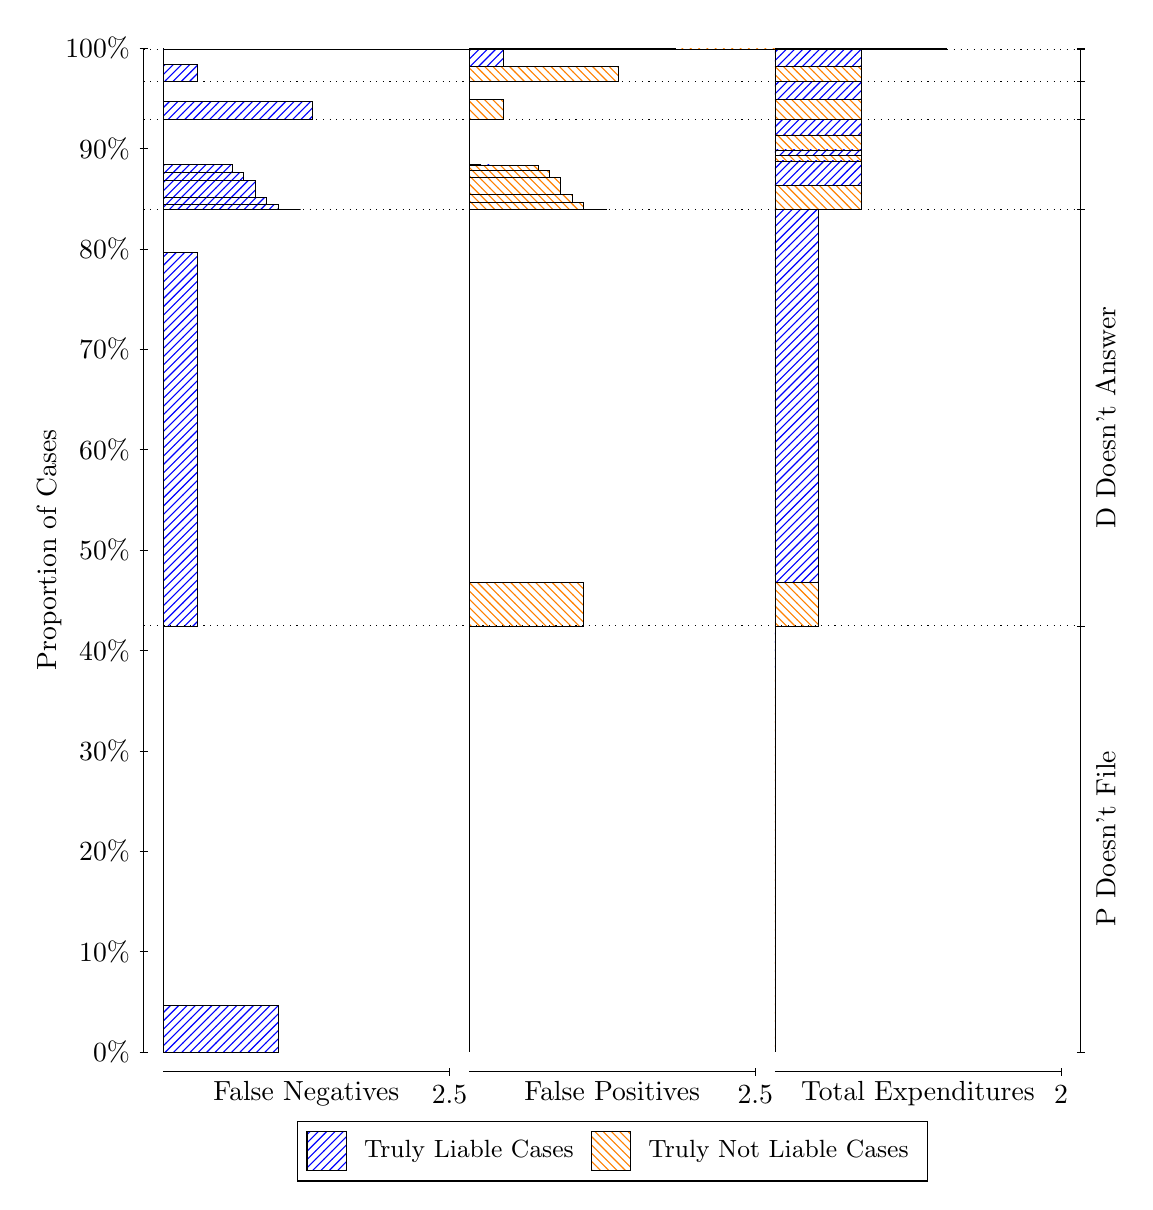
\begin{tikzpicture}
\draw[black, very thin] (1.5,1.75) -- (1.5,14.5);
\node[rotate=90, text=black, anchor=center] at (0.3, 8.125) {Proportion of Cases};
\draw[black, very thin] (1.45,1.75) -- (1.55,1.75);
\node[text=black, anchor=east] at (1.45, 1.75) {0\%};
\draw[black, very thin] (1.45,3.025) -- (1.55,3.025);
\node[text=black, anchor=east] at (1.45, 3.025) {10\%};
\draw[black, very thin] (1.45,4.3) -- (1.55,4.3);
\node[text=black, anchor=east] at (1.45, 4.3) {20\%};
\draw[black, very thin] (1.45,5.575) -- (1.55,5.575);
\node[text=black, anchor=east] at (1.45, 5.575) {30\%};
\draw[black, very thin] (1.45,6.85) -- (1.55,6.85);
\node[text=black, anchor=east] at (1.45, 6.85) {40\%};
\draw[black, very thin] (1.45,8.125) -- (1.55,8.125);
\node[text=black, anchor=east] at (1.45, 8.125) {50\%};
\draw[black, very thin] (1.45,9.4) -- (1.55,9.4);
\node[text=black, anchor=east] at (1.45, 9.4) {60\%};
\draw[black, very thin] (1.45,10.675) -- (1.55,10.675);
\node[text=black, anchor=east] at (1.45, 10.675) {70\%};
\draw[black, very thin] (1.45,11.95) -- (1.55,11.95);
\node[text=black, anchor=east] at (1.45, 11.95) {80\%};
\draw[black, very thin] (1.45,13.225) -- (1.55,13.225);
\node[text=black, anchor=east] at (1.45, 13.225) {90\%};
\draw[black, very thin] (1.45,14.5) -- (1.55,14.5);
\node[text=black, anchor=east] at (1.45, 14.5) {100\%};

\draw[black, very thin] (13.4,1.75) -- (13.4,14.5);
\draw[black, very thin] (13.35,1.75) -- (13.45,1.75);
\node[anchor=west] at (13.35, 1.75) {};
\draw[black, very thin] (13.35,7.1624) -- (13.45,7.1624);
\node[anchor=west] at (13.35, 7.1624) {};
\draw[black, very thin] (13.35,12.448) -- (13.45,12.448);
\node[anchor=west] at (13.35, 12.448) {};
\draw[black, very thin] (13.35,13.591) -- (13.45,13.591);
\node[anchor=west] at (13.35, 13.591) {};
\draw[black, very thin] (13.35,14.074) -- (13.45,14.074);
\node[anchor=west] at (13.35, 14.074) {};
\draw[black, very thin] (13.35,14.485) -- (13.45,14.485);
\node[anchor=west] at (13.35, 14.485) {};
\draw[black, very thin] (13.35,14.486) -- (13.45,14.486);
\node[anchor=west] at (13.35, 14.486) {};
\draw[black, very thin] (13.35,14.5) -- (13.45,14.5);
\node[anchor=west] at (13.35, 14.5) {};

\draw[black, very thin, pattern color=blue, pattern=north east lines] (1.75,1.75) rectangle (3.2033,2.3466);
\draw[black, very thin, pattern color=orange, pattern=north west lines] (1.75,2.3466) rectangle (1.75,7.1624);
\draw[black, very thin, pattern color=blue, pattern=north east lines] (1.75,7.1624) rectangle (2.186,11.901);
\draw[black, very thin, pattern color=orange, pattern=north west lines] (1.75,11.901) rectangle (1.75,12.448);
\draw[black, very thin, pattern color=blue, pattern=north east lines] (1.75,12.448) rectangle (3.494,12.448);
\draw[black, very thin, pattern color=blue, pattern=north east lines] (1.75,12.448) rectangle (3.3487,12.449);
\draw[black, very thin, pattern color=blue, pattern=north east lines] (1.75,12.449) rectangle (3.2033,12.517);
\draw[black, very thin, pattern color=blue, pattern=north east lines] (1.75,12.517) rectangle (3.058,12.517);
\draw[black, very thin, pattern color=blue, pattern=north east lines] (1.75,12.517) rectangle (3.058,12.604);
\draw[black, very thin, pattern color=blue, pattern=north east lines] (1.75,12.604) rectangle (2.9127,12.818);
\draw[black, very thin, pattern color=blue, pattern=north east lines] (1.75,12.818) rectangle (2.7673,12.924);
\draw[black, very thin, pattern color=blue, pattern=north east lines] (1.75,12.924) rectangle (2.622,13.019);
\draw[black, very thin, pattern color=blue, pattern=north east lines] (1.75,13.019) rectangle (2.4767,13.023);
\draw[black, very thin, pattern color=blue, pattern=north east lines] (1.75,13.023) rectangle (2.3313,13.027);
\draw[black, very thin, pattern color=orange, pattern=north west lines] (1.75,13.027) rectangle (1.75,13.591);
\draw[black, very thin, pattern color=blue, pattern=north east lines] (1.75,13.591) rectangle (3.6393,13.819);
\draw[black, very thin, pattern color=orange, pattern=north west lines] (1.75,13.819) rectangle (1.75,14.074);
\draw[black, very thin, pattern color=blue, pattern=north east lines] (1.75,14.074) rectangle (2.186,14.296);
\draw[black, very thin, pattern color=orange, pattern=north west lines] (1.75,14.296) rectangle (1.75,14.485);
\draw[black, very thin, pattern color=blue, pattern=north east lines] (1.75,14.485) rectangle (5.8193,14.485);
\draw[black, very thin, pattern color=orange, pattern=north west lines] (1.75,14.485) rectangle (1.75,14.486);
\draw[black, very thin, pattern color=orange, pattern=north west lines] (1.75,14.486) rectangle (1.75,14.489);
\draw[black, very thin, pattern color=blue, pattern=north east lines] (1.75,14.489) rectangle (1.75,14.5);
\draw[black, very thin, pattern color=orange, pattern=north west lines] (5.6333,1.75) rectangle (5.6333,6.5658);
\draw[black, very thin, pattern color=blue, pattern=north east lines] (5.6333,6.5658) rectangle (5.6333,7.1624);
\draw[black, very thin, pattern color=orange, pattern=north west lines] (5.6333,7.1624) rectangle (7.0867,7.7097);
\draw[black, very thin, pattern color=blue, pattern=north east lines] (5.6333,7.7097) rectangle (5.6333,12.448);
\draw[black, very thin, pattern color=orange, pattern=north west lines] (5.6333,12.448) rectangle (7.3773,12.449);
\draw[black, very thin, pattern color=orange, pattern=north west lines] (5.6333,12.449) rectangle (7.232,12.451);
\draw[black, very thin, pattern color=orange, pattern=north west lines] (5.6333,12.451) rectangle (7.0867,12.542);
\draw[black, very thin, pattern color=orange, pattern=north west lines] (5.6333,12.542) rectangle (6.9413,12.646);
\draw[black, very thin, pattern color=orange, pattern=north west lines] (5.6333,12.646) rectangle (6.796,12.858);
\draw[black, very thin, pattern color=orange, pattern=north west lines] (5.6333,12.858) rectangle (6.6507,12.944);
\draw[black, very thin, pattern color=orange, pattern=north west lines] (5.6333,12.944) rectangle (6.5053,13.012);
\draw[black, very thin, pattern color=orange, pattern=north west lines] (5.6333,13.012) rectangle (6.36,13.012);
\draw[black, very thin, pattern color=orange, pattern=north west lines] (5.6333,13.012) rectangle (6.2147,13.013);
\draw[black, very thin, pattern color=blue, pattern=north east lines] (5.6333,13.013) rectangle (5.924,13.016);
\draw[black, very thin, pattern color=blue, pattern=north east lines] (5.6333,13.016) rectangle (5.7787,13.021);
\draw[black, very thin, pattern color=blue, pattern=north east lines] (5.6333,13.021) rectangle (5.6333,13.591);
\draw[black, very thin, pattern color=orange, pattern=north west lines] (5.6333,13.591) rectangle (6.0693,13.847);
\draw[black, very thin, pattern color=blue, pattern=north east lines] (5.6333,13.847) rectangle (5.6333,14.074);
\draw[black, very thin, pattern color=orange, pattern=north west lines] (5.6333,14.074) rectangle (7.5227,14.262);
\draw[black, very thin, pattern color=blue, pattern=north east lines] (5.6333,14.262) rectangle (6.0693,14.485);
\draw[black, very thin, pattern color=orange, pattern=north west lines] (5.6333,14.485) rectangle (5.6333,14.485);
\draw[black, very thin, pattern color=blue, pattern=north east lines] (5.6333,14.485) rectangle (5.6333,14.486);
\draw[black, very thin, pattern color=orange, pattern=north west lines] (5.6333,14.486) rectangle (9.7027,14.489);
\draw[black, very thin, pattern color=blue, pattern=north east lines] (5.6333,14.489) rectangle (8.2493,14.5);
\draw[black, very thin, pattern color=orange, pattern=north west lines] (9.5167,1.75) rectangle (9.5167,6.5658);
\draw[black, very thin, pattern color=blue, pattern=north east lines] (9.5167,6.5658) rectangle (9.5167,7.1624);
\draw[black, very thin, pattern color=orange, pattern=north west lines] (9.5167,7.1624) rectangle (10.062,7.7097);
\draw[black, very thin, pattern color=blue, pattern=north east lines] (9.5167,7.7097) rectangle (10.062,12.448);
\draw[black, very thin, pattern color=orange, pattern=north west lines] (9.5167,12.448) rectangle (10.607,12.753);
\draw[black, very thin, pattern color=blue, pattern=north east lines] (9.5167,12.753) rectangle (10.607,13.067);
\draw[black, very thin, pattern color=orange, pattern=north west lines] (9.5167,13.067) rectangle (10.607,13.136);
\draw[black, very thin, pattern color=blue, pattern=north east lines] (9.5167,13.136) rectangle (10.607,13.206);
\draw[black, very thin, pattern color=orange, pattern=north west lines] (9.5167,13.206) rectangle (10.607,13.396);
\draw[black, very thin, pattern color=blue, pattern=north east lines] (9.5167,13.396) rectangle (10.607,13.591);
\draw[black, very thin, pattern color=orange, pattern=north west lines] (9.5167,13.591) rectangle (10.607,13.847);
\draw[black, very thin, pattern color=blue, pattern=north east lines] (9.5167,13.847) rectangle (10.607,14.074);
\draw[black, very thin, pattern color=orange, pattern=north west lines] (9.5167,14.074) rectangle (10.607,14.262);
\draw[black, very thin, pattern color=blue, pattern=north east lines] (9.5167,14.262) rectangle (10.607,14.485);
\draw[black, very thin, pattern color=orange, pattern=north west lines] (9.5167,14.485) rectangle (11.697,14.485);
\draw[black, very thin, pattern color=blue, pattern=north east lines] (9.5167,14.485) rectangle (11.697,14.486);
\draw[black, very thin, pattern color=orange, pattern=north west lines] (9.5167,14.486) rectangle (11.697,14.489);
\draw[black, very thin, pattern color=blue, pattern=north east lines] (9.5167,14.489) rectangle (11.697,14.5);
\draw[black, dotted] (1.5,7.1624) -- (13.4,7.1624);
\draw[black, dotted] (1.5,12.448) -- (13.4,12.448);
\draw[black, dotted] (1.5,13.591) -- (13.4,13.591);
\draw[black, dotted] (1.5,14.074) -- (13.4,14.074);
\draw[black, dotted] (1.5,14.485) -- (13.4,14.485);
\draw[black, dotted] (1.5,14.486) -- (13.4,14.486);
\draw[black, very thin] (1.75,1.5) -- (5.3833,1.5);
\node[text=black, anchor=north] at (3.5667, 1.5) {False Negatives};
\draw[black, very thin] (5.3833,1.45) -- (5.3833,1.55);
\node[text=black, anchor=north] at (5.3833, 1.45) {2.5};

\draw[black, very thin] (5.6333,1.5) -- (9.2667,1.5);
\node[text=black, anchor=north] at (7.45, 1.5) {False Positives};
\draw[black, very thin] (9.2667,1.45) -- (9.2667,1.55);
\node[text=black, anchor=north] at (9.2667, 1.45) {2.5};

\draw[black, very thin] (9.5167,1.5) -- (13.15,1.5);
\node[text=black, anchor=north] at (11.333, 1.5) {Total Expenditures};
\draw[black, very thin] (13.15,1.45) -- (13.15,1.55);
\node[text=black, anchor=north] at (13.15, 1.45) {2};

\node[text=black, centered, rotate=90] at (13.72, 4.4562) {P Doesn't File};
\node[text=black, centered, rotate=90] at (13.72, 9.8052) {D Doesn't Answer};






\draw (7.449999999999999,1.5) node[draw=none] (baseCoordinate) {};
\begin{scope}[align=center]
        \matrix[scale=0.5, draw=black, below=0.5cm of baseCoordinate, nodes={draw}, column sep=0.1cm]{
            \node[rectangle, draw, minimum width=0.5cm, minimum height=0.5cm, pattern color=blue, pattern=north east lines] {}; &
            \node[draw=none, font=\small, text=black] (B) {Truly Liable Cases}; &
            \node[rectangle, draw, minimum width=0.5cm, minimum height=0.5cm, pattern color=orange, pattern=north west lines] {}; &
            \node[draw=none, font=\small, text=black] (B) {Truly Not Liable Cases}; \\
            };
\end{scope}

\end{tikzpicture}
\end{document}